\documentclass{article} % For LaTeX2e
\usepackage{nips14submit_e,times}
\usepackage{amsmath}
\usepackage{amsthm}
\usepackage{amssymb}
\usepackage{mathtools}
\usepackage{hyperref}
\usepackage{url}
\usepackage{algorithm}
\usepackage[noend]{algpseudocode}
%\documentstyle[nips14submit_09,times,art10]{article} % For LaTeX 2.09

\usepackage{mathrsfs}
\usepackage{graphicx}
\usepackage{caption}
\usepackage{subcaption}

\def\eQb#1\eQe{\begin{eqnarray*}#1\end{eqnarray*}}
\def\eQnb#1\eQne{\begin{eqnarray}#1\end{eqnarray}}
\providecommand{\e}[1]{\ensuremath{\times 10^{#1}}}
\providecommand{\pb}[0]{\pagebreak}


\def\Qb#1\Qe{\begin{question}#1\end{question}}
\def\Sb#1\Se{\begin{solution}#1\end{solution}}

\newenvironment{claim}[1]{\par\noindent\underline{Claim:}\space#1}{}
\newtheoremstyle{quest}{\topsep}{\topsep}{}{}{\bfseries}{}{ }{\thmname{#1}\thmnote{ #3}.}
\theoremstyle{quest}
\newtheorem*{definition}{Definition}
\newtheorem*{theorem}{Theorem}
\newtheorem*{lemma}{Lemma}
\newtheorem*{question}{Question}
\newtheorem*{preposition}{Preposition}
\newtheorem*{exercise}{Exercise}
\newtheorem*{challengeproblem}{Challenge Problem}
\newtheorem*{solution}{Solution}
\newtheorem*{remark}{Remark}
\usepackage{verbatimbox}
\usepackage{listings}

\title{Real Variables: \\
Problem Set XI}


\author{
Youngduck Choi \\
Courant Institute of Mathematical Sciences \\
New York University \\
\texttt{yc1104@nyu.edu} \\
}


% The \author macro works with any number of authors. There are two commands
% used to separate the names and addresses of multiple authors: \And and \AND.
%
% Using \And between authors leaves it to \LaTeX{} to determine where to break
% the lines. Using \AND forces a linebreak at that point. So, if \LaTeX{}
% puts 3 of 4 authors names on the first line, and the last on the second
% line, try using \AND instead of \And before the third author name.

\newcommand{\fix}{\marginpar{FIX}}
\newcommand{\new}{\marginpar{NEW}}

\nipsfinalcopy % Uncomment for camera-ready version

\begin{document}


\maketitle

\begin{abstract}
This work contains solutions to the problem set 
XI of Real Variables 2015 at NYU.
\end{abstract}

\section{Solutions}

\begin{question}[Royden 17-6]
\hfill
\begin{figure}[h!]
  \centering
    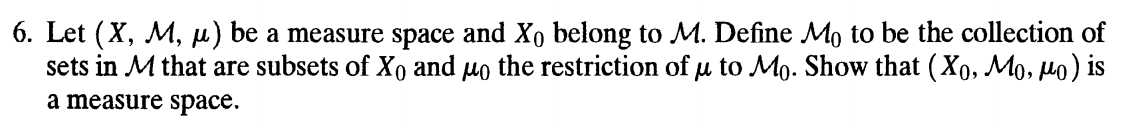
\includegraphics[width=1\textwidth]{rv-17-6.png}
\end{figure}
\end{question}
\begin{solution} 
We first show that $(X_0, \mathscr{M}_0)$ is a measurable space. To this
end, we must show that $\mathscr{M}_0$ is a $\sigma$-algebra of $X_0$.
As $\emptyset$ and $X_0$ belong to $\mathscr{M}$, are subsets of $X_0$,
it follows that $\emptyset$ and $X_0$ belong to $\mathscr{M}_0$. Let 
$\{A_n\}_{n=1}^{\infty}$ be a countable collections of sets in $\mathscr{M}_0$.
As $A_n \subseteq X_0$ for all $n$, we have $\bigcup_{n=1}^{\infty} A_n
\subseteq X_0$. Furthermore, as $\mathscr{M}$ is a $\sigma$-algebra, 
and $A_n \in \mathscr{M}$ for all $n$, we 
also have $\bigcup_{n=1}^{\infty} A_n \in \mathscr{M}$. Hence, it follows
that $\bigcup_{n=1}^{\infty} A_n \in \mathscr{M}_0$. Now, let $A$ be a 
set, belonging to $\mathscr{M}_0$. Then, 
as $X_0 \setminus A$ is a subset of
$X_0$, and $X_0$ and $A$ belong to $M$, which gives $X_0 \setminus A 
\in \mathscr{M}$, we have $X_0 \setminus A$ belongs to $\mathscr{M}_0$.
Hence, we have shown that $\mathscr{M}_0$ is a $\sigma$-algebra, and
$(X_0, \mathscr{M}_0)$ is a measurable space. Now, it remains to be
shown that the restricted map $\mu_0$ has the properties of a measure.
First, observe that $\emptyset \in \mathscr{M}_0$ and $\mu_0(\emptyset)
= \mu(\emptyset) = 0$. Now, let $\{A_n\}$ be a countable disjoint sets 
from $\mathscr{M}_0$. Since $A_n \in \mathscr{M}$ for all $n$,
by the countable additivity of $\mu$ and the fact that $\mathscr{M}_0$
is a $\sigma$-algebra,
it follows that 
\eQb
\sum_{n=1}^{\infty} \mu_0 (A_n) &=& \sum_{n=1}^{\infty} \mu(A_n) \\
&=& \mu(\bigcup_{n=1}^{\infty} A_n ) \\
&=& \mu_0(\bigcup_{n=1}^{\infty} A_n). \\
\eQe
Therefore, we have shown that $(X_0, \mathscr{M}_0, \mu_0)$ is
a measure space. \hfill $\qed$
 
\end{solution}

\newpage

\begin{question}[Royden 17-15]
\hfill
\begin{figure}[h!]
  \centering
    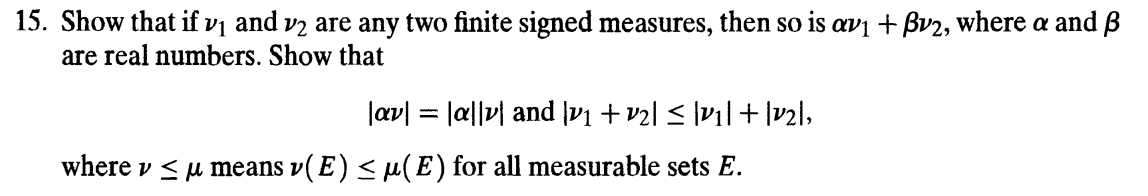
\includegraphics[width=1\textwidth]{rv-17-15.png}
\end{figure}
\end{question}
\begin{solution}
Let $(X,\mathscr{M})$ be a measurable space. 
Let $v_1$ and $v_2$ be two finite signed measures on $(X,\mathscr{M})$.
Consider a set function $\alpha v_1 + \beta v_2$ on $\mathscr{M}$,
 for $\alpha , \beta \in \mathbb{R}$,
which is defined by
\eQb
\alpha v_1 + \beta v_2(E) &=& \alpha v_1(E) + \beta v_2(E), 
\eQe
for $E \in \mathscr{M}$. As $v_1$ and $v_2$ only take finite values,
it also follows that $\alpha v_1 + \beta v_2$ also assumes only finite values,
as an addition of two finite values are finite. Furthermore, it follows
that 
\eQb
\alpha v_1 + \beta v_2(\emptyset) &=& \alpha v_1(\emptyset) + 
\beta v_2(\emptyset) \\
&=& 0 + 0 = 0,  
\eQe
as $v_1$ and $v_2$ are signed measures. Furthermore, the countable 
additivity property holds, as for any countable disjoint collection
$\{ E_k\}$ from $\mathscr{M}$, by linearity of limit, and countable
additivity of $v_1$ and $v_2$, it follows that
\eQb
\alpha v_1 + \beta v_2(\bigcup_{k=1}^{\infty} E_k) &=& 
\alpha v_1(\bigcup_{k=1}^{\infty} E_k) + \beta v_2(\bigcup_{k=1}^{\infty}
E_k) \\
&=& \alpha \sum_{k=1}^{\infty} v_1(E_k) + \beta \sum_{k=1}^{\infty} 
v_2(E_k) \\
&=& \sum_{k=1}^{\infty} \alpha v_1(E_k) + \beta v_2(E_k) \\
&=& \sum_{k=1}^{\infty} \alpha v_1 + \beta v_2(E_k).
\eQe  
Hence $\alpha v_1 + \beta v_2$ is a finite measure. 

\smallskip

Let $(X,\mathscr{M})$ be a measurable space and $v$ be a finite 
measure on the space. Consider $|\alpha v|$. It follows that
for $E \in \mathscr{M}$, we have
\eQb
|\alpha v(E)| &=& |\alpha||v(E)|.
\eQe  
Hence, $|\alpha v| = |\alpha| |v|$. Now, let $v_1$ and $v_2$ be 
finite signed measures on $(X,\mathscr{M})$. By the triangle
inequality of reals, it follows that for any $E \in \mathscr{M}$,
\eQb
|v_1 + v_2(E)| &=& |v_1(E) + v_2(E)| \\
&\leq& |v_1(E)| + |v_2(E)| . 
\eQe 
Hence, $|v_1 + v_2| \leq |v_1| + |v_2|$. \hfill $\qed$
\end{solution}

\newpage

\begin{question}[Royden 17-17]
\hfill
\begin{figure}[h!]
  \centering
    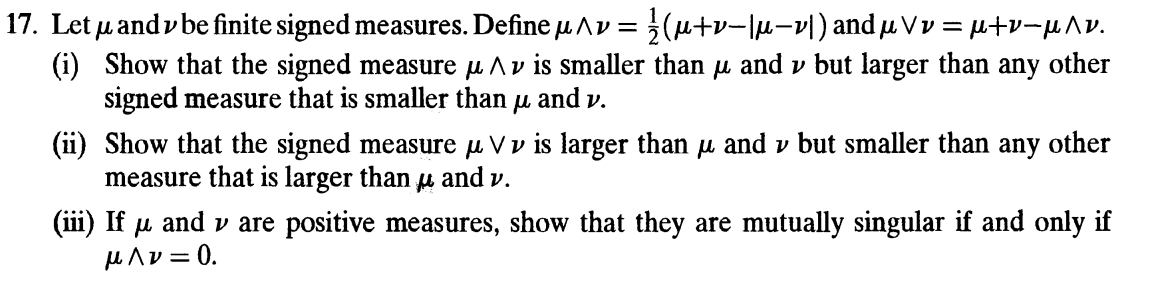
\includegraphics[width=1\textwidth]{rv-17-17.png}
\end{figure}
\end{question}
\begin{solution}
\textbf{(i)} Let $u$ and $v$ be finite signed measures on $(X,\mathscr{M})$.
We wish to show that $u \wedge v \leq u$. By writing out $u \wedge v$
term, multiplying by $2$, and re-arranging the terms trivially, we see that
$u \wedge v \leq u$ is equivalent to $u - v \leq |u-v|$. As an absolute
value of a real number is larger than the number itself, we see that
$u \wedge v \leq u$ holds. By symmetry, we also see that $u \wedge v 
\leq v$ as well.  

\smallskip

Now, let $t$ be a signed measure such that $t \leq u$ and $t \leq v$.
It follows that $t \leq \min(u,v)$. Assume without loss of generality that
$\min(u,v) = u$. It follows that
\eQb
\dfrac{1}{2}(u + v |u-v|) &=& \dfrac{1}{2}(2u) \\
&=& u. 
\eQe
Therefore, $\min(u,v) = \dfrac{1}{2}(u + v - |u - v|)$. 
Hence, $t \leq u \wedge v $.

\smallskip

\textbf{(ii)} Let $u$ and $v$ be finite signed measures on $(X,
\mathscr{M})$. In the above
solution, we have shown that $u \wedge v = \min(u,v)$. Hence, it follows
that $u + v - u \wedge v = \max(u,v)$. Therefore, we obtain that 
$u \lor v \geq u$ and $u \lor v \geq v$. Again, as for any $t$ such that
$t \geq u$ and $t \geq v$, it follows that $t \geq \max(u,v) = u \lor v$. 
 
\smallskip
 
\textbf{(iii)} Let that $u$ and $v$ are finite measures, and 
assume that $u \wedge v  = \dfrac{1}{2}(u+v - |u-v|) =  0$. 
For any $E \in \mathscr{M}$, it follows that
\eQb
u(E) + v(E) = |u(E) - v(E)| \\
\eQe
Suppose that $u(E)$ and $v(E)$ are both strictly positive. It follows that
$u(E) + v(E) > \max(u(E), v(E))$ and $|u(E) - v(E) < \max(u(E),v(E))$,
which yields a contradiction with the above equality. Hence, we have that
at least one of $u(E)$ or $v(E)$ is 0. Assume without loss of generality that
$u(E) = 0$. Now, with the same argument with respect to $E^c$, it follows 
that either $u(E^c)$ and $v(E^c)$ is $0$. If $v(E^c) = 0$, then $u$ and $v$
are mutually singular. Now, consider the remaining case of $u(E^c) = 0$. 
By the additivity property of a signed measure, we have that 
$u(X) = 0$. Hence, $u(X) = 0$ and $v(\emptyset) = 0$. Therefore, we 
have shown that $u$ and $v$ are mutually singular. 

\smallskip

Now, assume that $u$ and $v$ are mutually singular measures. 
Hence, there exists a disjoint measurable set $A$ and $B$ such that
$A \cup B = X$ and $u(A) = 0$ and $v(B) = 0$. Let $E \in \mathscr{M}$.
Then, it follows that
\eQb
u\wedge v(E) &=& u \wedge v (E \cap A) + u \wedge v (E \cap B) \\
&=&  \dfrac{1}{2}(u + v - |u-v|)(E \cap A) + 
\dfrac{1}{2}(u + v - |u-v|)(E \cap B) \\ 
&=& 0 + 0,
\eQe 
by the monotonicity property. 
 

\hfill $\qed$ 

\end{solution}

\newpage

\begin{question}[Royden 18-50]
\hfill
\begin{figure}[h!]
  \centering
    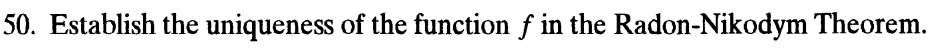
\includegraphics[width=1\textwidth]{rv-18-50.png}
\end{figure}
\end{question}
\begin{solution}
Let $(X,\mathscr{M})$ be a measurable space, and $u$, $v$ be $\sigma$-finite
measures on the space with $v << u$.
Let $f$ and $g$ be the non-negative measurable functions for which,
\eQb
v(E) &=& \int_{E} f du \\
&=& \int_{E} g du,
\eQe
for all $E \in \mathscr{M}$. By the linearity of integration for non-negative
measures, we obtain that
\eQb
\int_{E} f - g du &=& 0,
\eQe
for all $E \in \mathscr{M}$. Now, we prove that if $\int_{E} f du = 0$
for every measurable subset $E$ of $X$, then $f = 0$ a.e. on $X$. We 
prove the case for $f$ non-negative and the result can be extended through
an argument with $f^+$ and $f^-$ decomposition. Define $A_n = \{ x \in X \>
| \> f(x) \geq \dfrac{1}{n} \}$. we have $\cup_{n} A_n = \{ x \in X \> |
\> f(x) > 0\}$. Now, observe that by the assumption, $ \int_{A_n}f du
= 0$ for all $n$ and $\dfrac{1}{n} u(A_n) \leq 
\int_{A_n} f du = 0$, which gives $u(A_n) = 0$ for all $n$. Therefore,
by the countable additivity,
we obtain that $u(\cup_{n} A_n) = 0$. Hence, we have shown that
$f = 0$ a.e. Therefore, we have that $f -g$ from the Radon-Nikodym theorem,
must be $0$ a.e. on $X$. Hence, we have shown the uniqueness of Radon-Nikodym
theorem.
\hfill $\qed$
 

\end{solution}

\newpage

\begin{question}[Royden 18-54]
\hfill
\begin{figure}[h!]
  \centering
    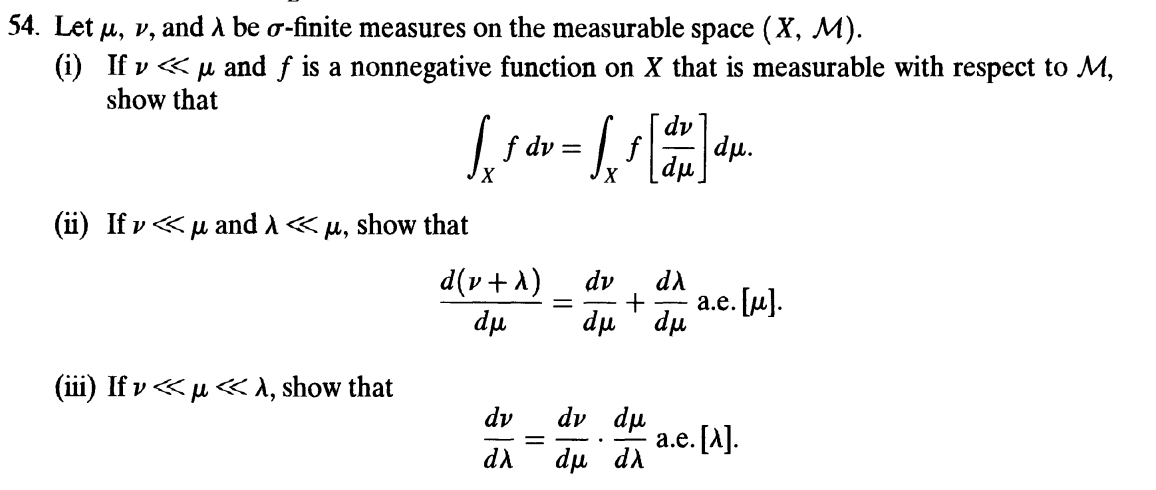
\includegraphics[width=1\textwidth]{rv-18-54.png}
\end{figure}
\end{question}
\begin{solution}

\end{solution}
\newpage

\begin{question}[Royden 18-55]
\hfill
\begin{figure}[h!]
  \centering
    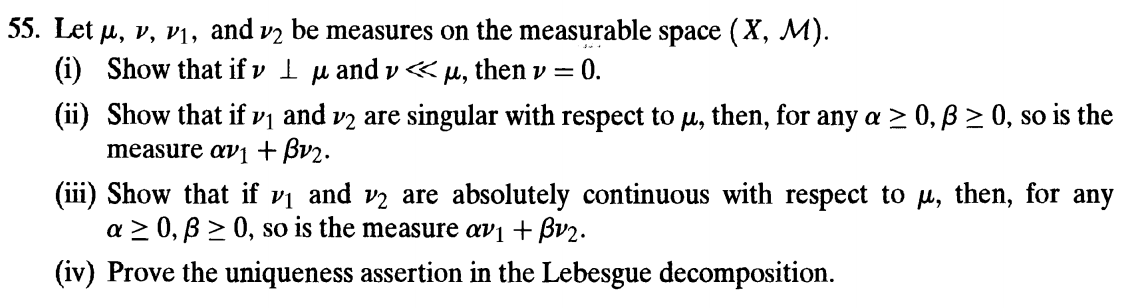
\includegraphics[width=1\textwidth]{rv-18-55.png}
\end{figure}
\end{question}
\begin{solution}
\textbf{(i)} Assume $v \perp u$, and $ v << u$. It follows that
there exists a pair of measurable sets $A$ and $B$ such that 
$u(A) = 0$ and $v(B) = 0$. By the absolute continuity of $v$ with respect
to $u$, it follows that $v(A) = 0$. By finite additivity of measure, we
obtain that $v(X) = 0$. In other words, $v$ is a zero measure.

\smallskip

\textbf{(ii)} 
Assume $u \perp v$. We show that $u \perp \alpha v$, for $\alpha \geq 0$
holds as well.
As $u \perp v$, there exists $A$ and $B$ from $\mathscr{M}$ such that
$u(A) = 0$ and $v(B) = 0$ and $A \cup B = X$. Observe that
$\alpha v(B) = 0$ as well. Hence, $u \perp \alpha v$. Now, assume
$u \perp v_1$ and $u \perp v_2$. We show that $u \perp v_1 + v_2$.
Let $(A_1, B_1)$ and $(A_2,B_2)$ be the pairs of sets that grant
the mutual singularities. Then, observe that by finite additivity of 
measure, we have $u(A_1 \cup A_2) = 0$. Furthermore, observe that
by monotonicity of measure, $v_1 + v_2(B_1 \cap B_2) = 0$. Since
$A_1 \cup A_2 \cup (B_1 \cap B_2) = (A_1 \cup A_2 \cup B_1) \cap
(A_1 \cup A_2 \cup B_2) = X \cap X = X$, we have that $u$ and $v_1 + v_2$
are mutually singular. Hence, the claim is proven. 

\smallskip

\textbf{(iii)} 
Assume $v << u$. Then, for any $E \in \mathscr{M}$ such that
$u(E) = 0$, we have $v(E) = 0$. Since $v(E) = 0
$, we also have $\alpha v(E) = 0$. Hence, $\alpha v << u$. Now, 
assume $v_1 << u$ and $v_2 << u$. It follows that for any 
$E \in \mathscr{M}$ such that $u(E) = 0$, we have $v_1(E) = 0$ and
$v_2(E) = 0$. Therefore, $v_1+v_2(E) = 0$. Hence, the claim is proven.

\bigskip

\textbf{(iv)} Let $v_0$ and $v_1$ be the Lebesque decomposition measures,
where $v_0$ is mutually singular and $v_1$ is absolutely continuous with
respect to $v_1$. Consider $v^{'}_0$ and $v^{'}_1$ with the same set-up.
We have that $v_0 + v_1 = v^{'}_0 + v^{'}_1$. It follows that
\eQb
v_0 - v^{'}_0 &=& v_1 - v^{'}_1.
\eQe  
Observe that $v_0 - v^{'}_0$ and $v_1 - v^{'}_1$ are singular and
absolutely continuous with respect to $u$ from $(ii)$ and $(iii)$. 
Hence, by $(i)$, we have that $v_0 = v^{'}_0$ and $v_1 = v^{'}_0$.
Therefore, we have shown that uniqueness of the decomposition. 
\hfill $\qed$
 

\end{solution}

\end{document}
